\documentclass{scrreprt}
\usepackage[bookmarks=true]{hyperref}
\usepackage{tabto}
\usepackage{epsfig}
\usepackage{epstopdf}
\hypersetup{
    pdftitle={Functional Requirement Specification},    % title
    colorlinks=true,       % false: boxed links; true: colored links
    linkcolor=blue,       % color of internal links
    citecolor=black,       % color of links to bibliography
    filecolor=black,        % color of file links
    urlcolor=purple,        % color of external links
    linktoc=page            % only page is linked
}%
\title{%
\author{
Khathutshelo Matidza 11072157\\
\and
Renaldo van Dyk 12204359\\
\and
Andreas du Preez 12207871\\
\and
Sean Hill 12221458\\
\and
Kgomotso Sito 12243273\\
\and
Hlavutelo Maluleke 12318109\\
\and
Sboniso Masilela 10416260\\
\and
Semaka Malapane 13081129\\
}
\centering
\Huge{FUNCTIONAL REQUIREMENTS\\ SPECIFICATION}\\
\vspace{2cm}
FOR\\
\vspace{2cm}
Buzz System\\
\vspace{2cm}
Mini Project Phase 1\\
GitHub\\
\LARGE\texttt{https://github.com/RenaldoV/COS301\_Group5\_a}
\vfill
\vspace{1cm}
\rule{15cm}{3pt}
}
\date{}
\usepackage{hyperref}
\begin{document}
\maketitle
\tableofcontents
\chapter{ Introduction}
This document discusses the application functionality required by users (and other stakehodlers).\\
\chapter{Searching and Filtering}
\section{Use case prioritization}
\subsection{Critical}
1.1 Search\\
1.1.1 Search for student\\
1.1.1.1 Search by name\\
1.1.1.2 Search by student number\\
1.1.2 Search for posts\\
1.1.2.1 Search posts by title\\

\subsection{Important}
1.2 Filter posts\\
1.2.1 Filter by title\\
1.2.2 Filter by module code\\

\subsection{Nice-To-Have}
1.2.3 Filter by user\\
1.2.3 Filter by date\\

\section{Use case/Services contracts}
\subsection{Pre-Conditions}								%PRE CONDITIONS
1.1	Search text is invalid\\
1.1.1	Student does not exist in system\\
1.1.1.1	Student of specified name does not exist in the system\\
1.1.1.2	Student of specified student number does not exist in system\\
1.1.2	Post does not exist\\
1.1.2.1	Post of specified title does not exist\\
\newline
1.2	a) Criteria to filter is invalid\\
b) No posts available to filter\\
1.2.1	Invalid title specified\\
1.2.2	Module code does not exist\\
1.2.3	a) Incorrect user specified
b) User does not exist\\
1.2.4	a) Date incorrectly specified\\
\subsection{Post-Conditions}%POST CONDITIONS	
1.1	Search results returned\\
1.1.1	Student details of student searched for are returned\\
1.1.1.1	Student details of student number specified are returned\\
1.1.2	Post searched for is returned\\
1.1.2.1	Post of specified title is returned\\

\section{Request and Results Data Structures} 
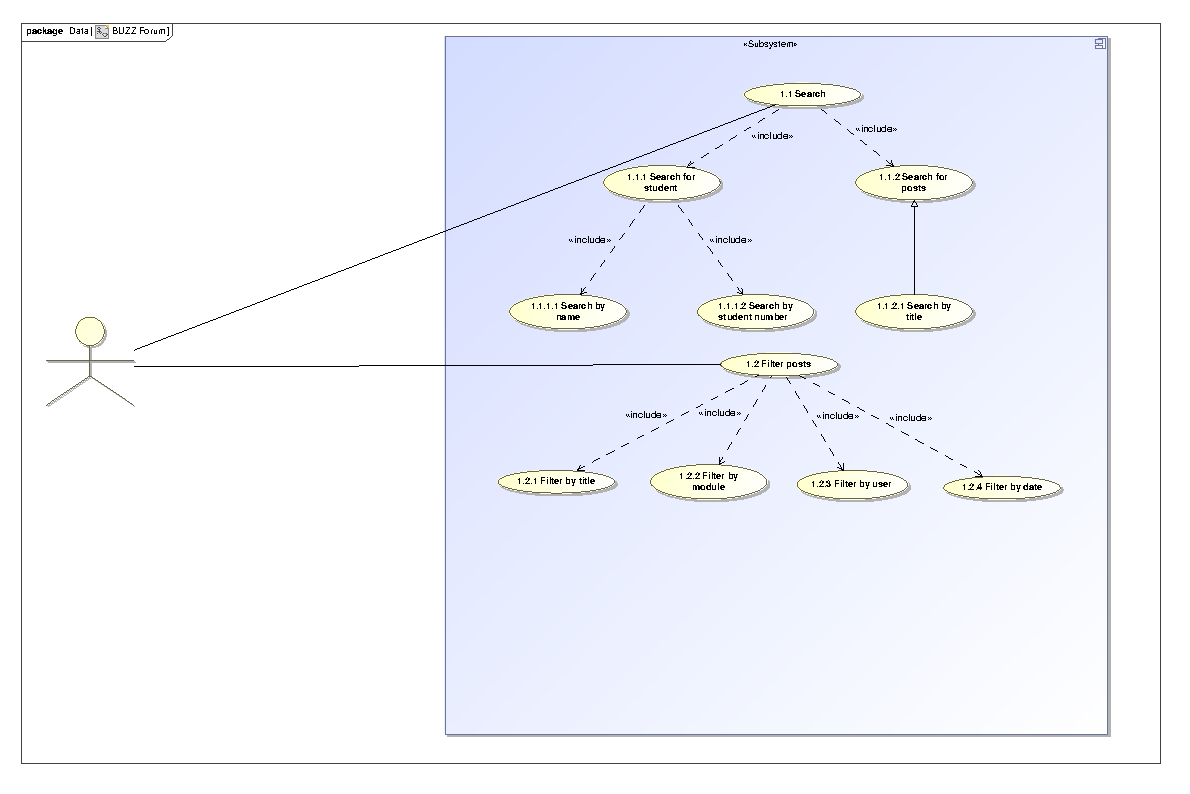
\includegraphics[scale=.9]{graphics/searchAndFilterUseCase.eps}\\

\section{Process specifications}
\subsection{Search}
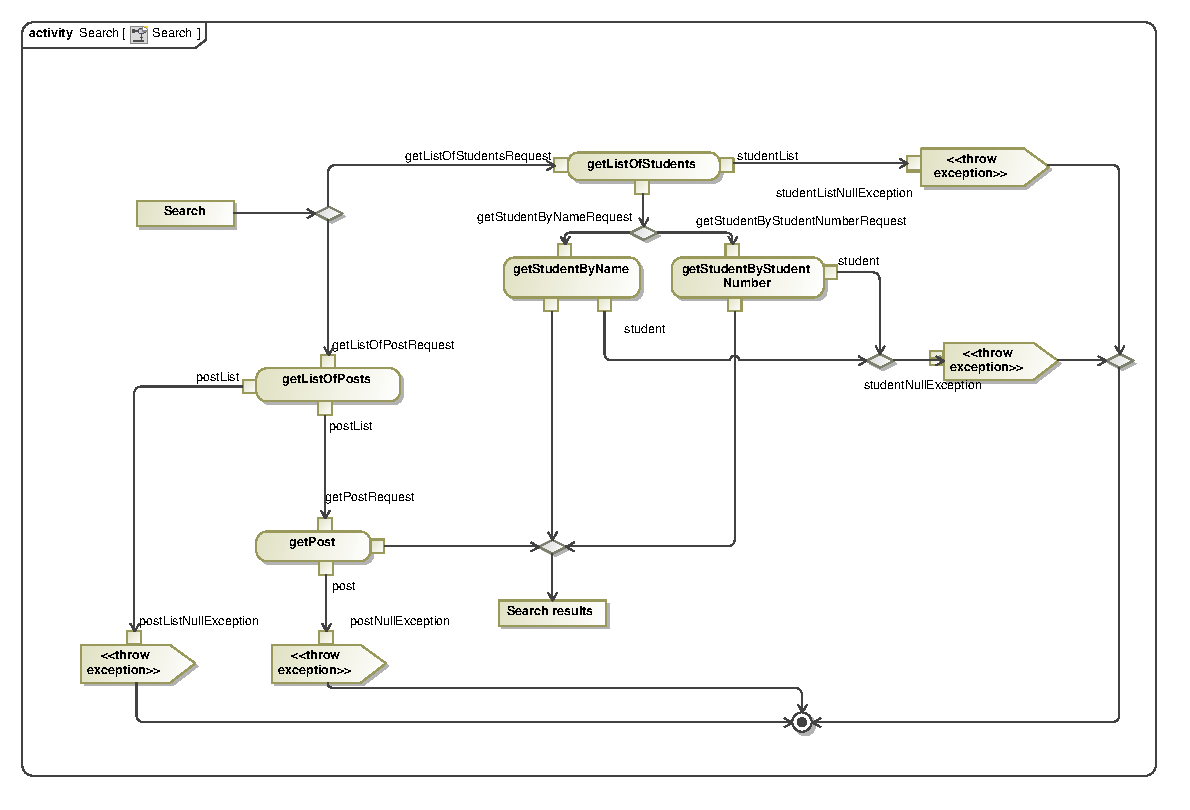
\includegraphics[scale=.9]{graphics/searchActivityDiagram.eps}\\
\subsection{Filter}
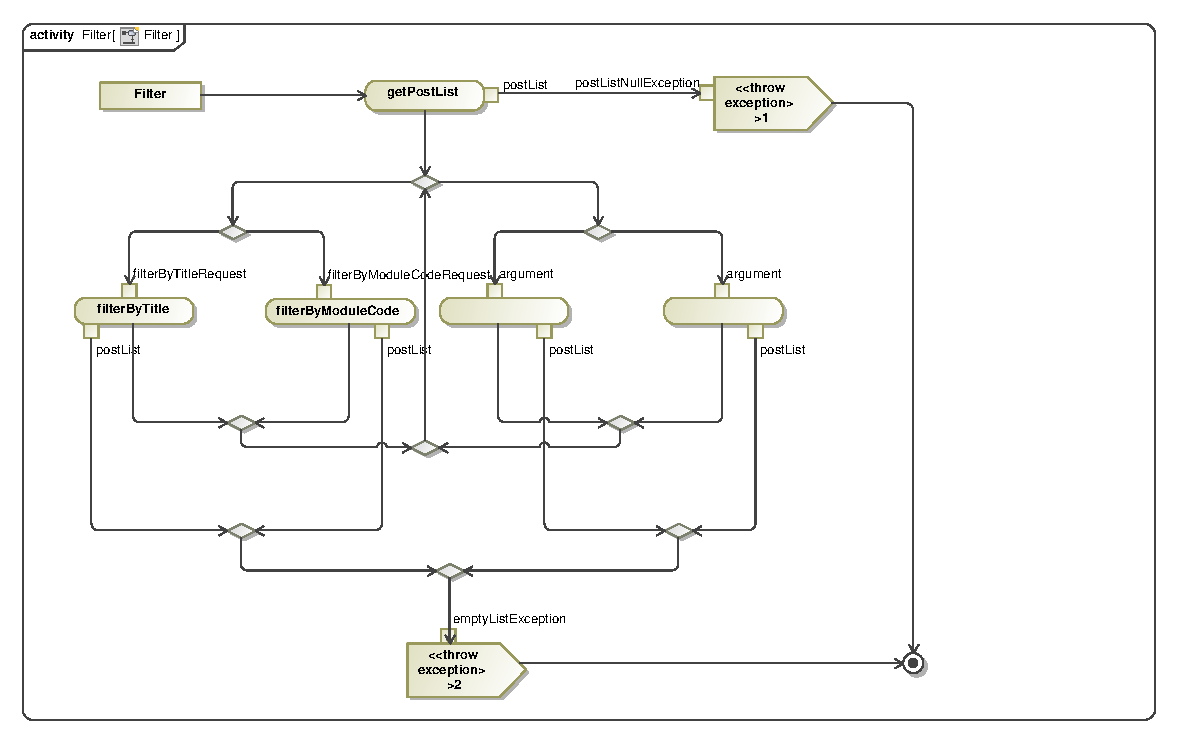
\includegraphics[scale=.9]{graphics/filterActivityDiagram.eps}\\

\section{Domain Model} 
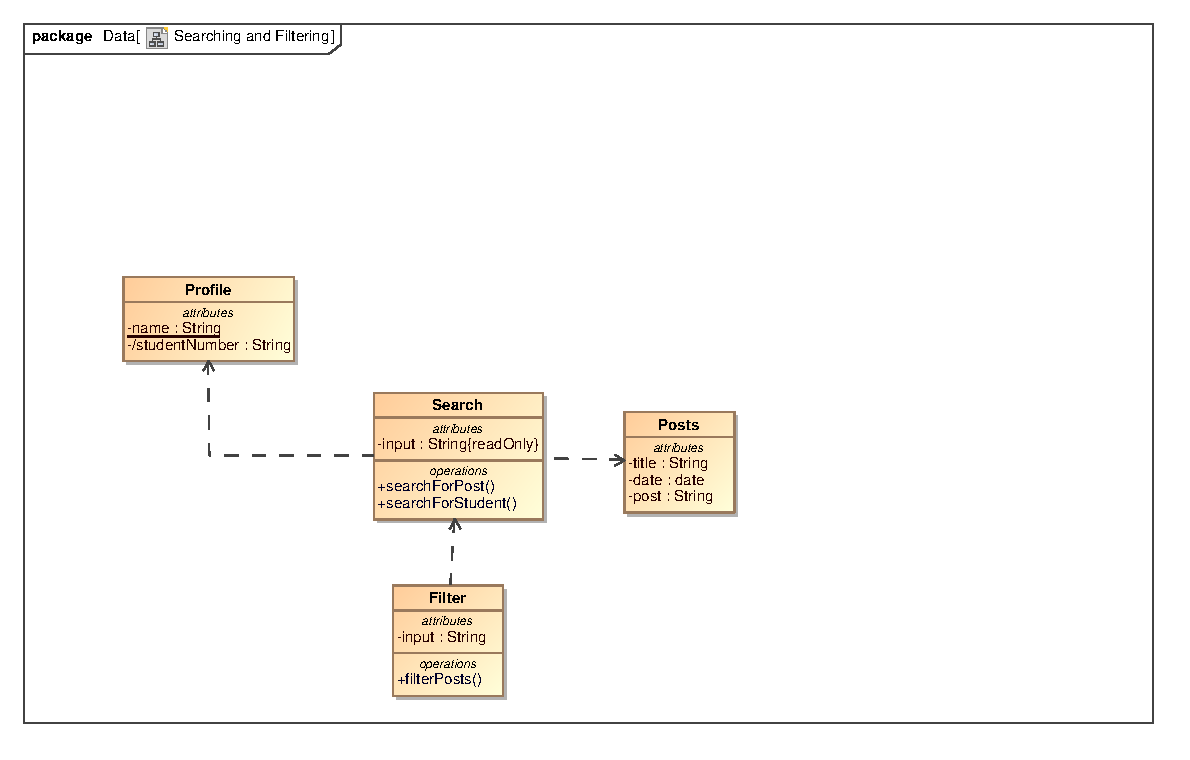
\includegraphics[scale=.9]{graphics/searchAndFilterUML.eps}\\

\chapter{Rating}
\section{Use case prioritization}
\subsection{Critical}
1.2	Rate\\
1.1.1 Like comment\\
1.1.2 Dislike comment\\
1.1.3 Store rating\\

\subsection{Important}

\subsection{Nice-To-Have}

\section{Use case/Services contracts}
\subsection{Pre-Conditions}								%PRE CONDITIONS
1.2	User not logged in\\
1.1.1 Post does not exist\\
1.1.2 Post does not exist\\
1.1.3 Rating invalid\\

\subsection{Post-Conditions}%POST CONDITIONS	
1.2	User not logged in\\
1.1.1 Post does not exist\\
1.1.2 Post does not exist\\
1.1.2 Rating invalid\\

\section{Request and Results Data Structures} 
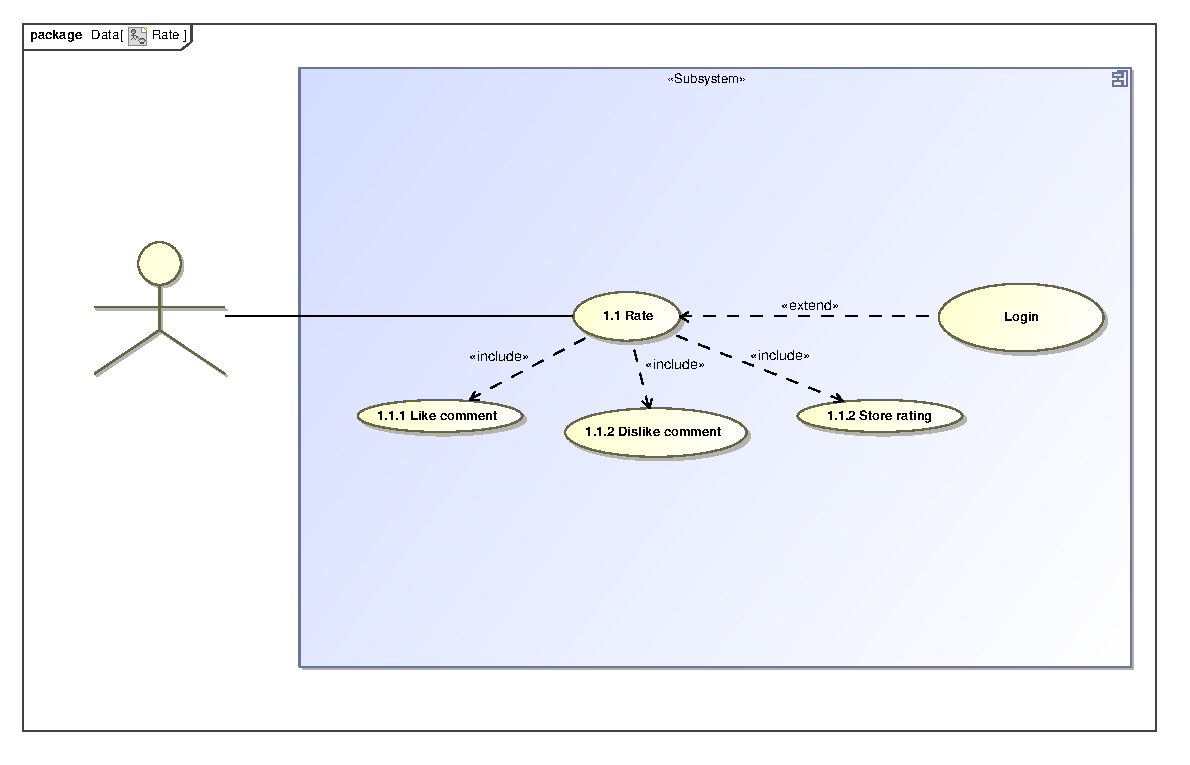
\includegraphics[scale=.9]{graphics/rateUseCase.eps}\\

\section{Process specifications}
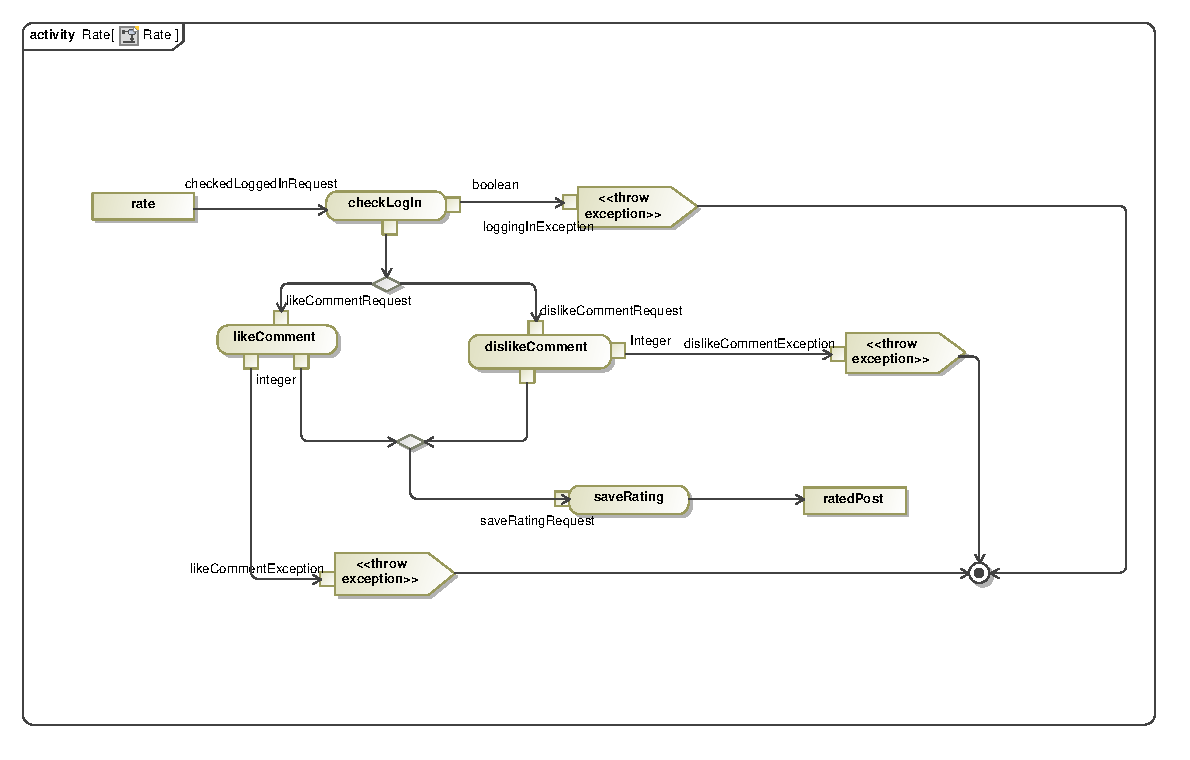
\includegraphics[scale=.9]{graphics/rateActivityDiagram.eps}\\

\section{Domain Model} 
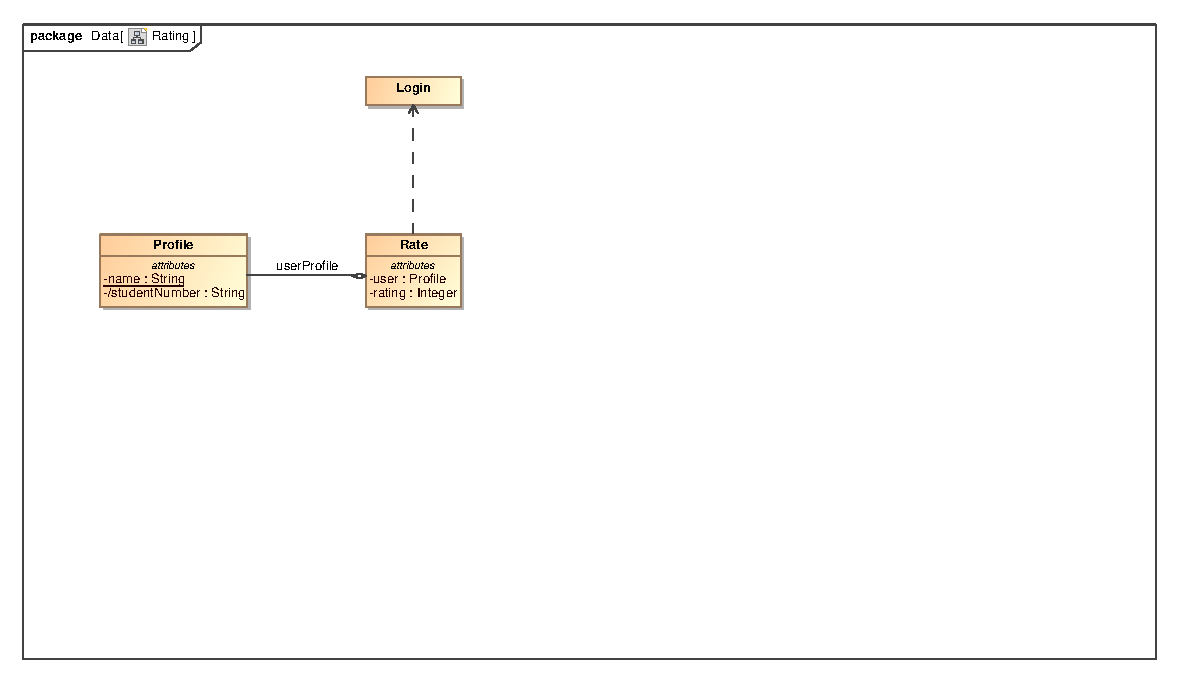
\includegraphics[scale=.9]{graphics/rateUML.eps}\\	
% add other chapters and sections to suit
\end{document}